\documentclass[a4paper,12pt]{article}
\usepackage[utf8x]{inputenc}

%opening
\title{COSC 625 Final}
\author{Byron Heads \\
		E00062946}
\date{\today}
\usepackage{graphics}
\usepackage{listings}

\begin{document}
\maketitle

\section{}
\subsection{}
\begin{figure}[h!]
\center{\resizebox{380px}{!}{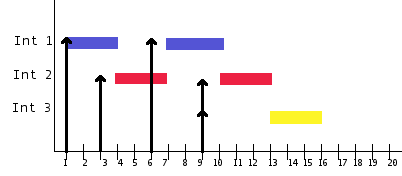
\includegraphics{1a.png}}}
\end{figure}

\subsection{}
\begin{tabular}{l | l | l | l }
Device & Trigger Time & Finish Time & Response Time \\ \hline
1 & 1 & 4 & 3 \\
2 & 3 & 7 & 4 \\
1 & 6 & 10 & 4 \\
2 & 9 & 13 & 4 \\
3 & 9 & 16 & 7 \\
& & &  4.4
\end{tabular}

\newpage
\subsection{}
\begin{figure}[h!]
\center{\resizebox{380px}{!}{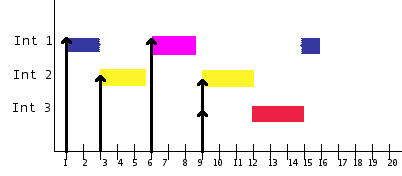
\includegraphics{1c.png}}}
\end{figure}

\subsection{}
\begin{tabular}{l | l | l | l }
Device & Trigger Time & Finish Time & Response Time \\ \hline
1 & 1 & 16 & 17 \\
2 & 3 & 6 & 3 \\
1 & 6 & 9 & 3 \\
2 & 9 & 12 & 3 \\
3 & 9 & 15 & 6 \\
& & &  6.4
\end{tabular}



\section{}
\subsection{}
\begin{figure}[h!]
\center{\resizebox{380px}{!}{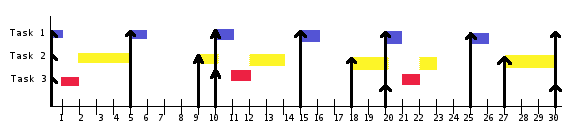
\includegraphics{2a.png}}}
\end{figure}

\subsection{}
90

\subsection{}
\begin{tabular}{l l}
Task & Average Response Time \\ \hline
1 & 1 \\
2 & 4.5 \\
3 & 2
\end{tabular}

\subsection{}

As long as all of the average response times for all of the task is well below the Period, then all of your tasks will happen within the Period.  You will have no missed tasks.

\section{}

\subsection{}
Ticks 2 to 3 and 7 to 8.
\begin{figure}[h!]
\center{\resizebox{380px}{!}{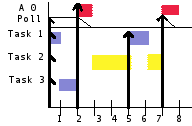
\includegraphics{3a.png}}}
\end{figure}

\subsection{}
Response time of 6.

\subsection{}
You could increase the capacity to 2.  Your response time would become 2.

\section{}
\lstset{language=C}
\begin{lstlisting}
27 #define NUM_TIMERS 1    /* number of timers */
28 #define NUM_TASKS  4    /* number of tasks  */
98 unsigned timers[NUM_TIMERS] = { 0 };
99 void (*timer[NUM_TIMERS]) (void)={tmr0};
111 unsigned task_flag[NUM_TASKS] = {0,0,0,IN_PROC};
112 void (*task[NUM_TASKS])(void) = {task0,task1,task2,main};
\end{lstlisting}

\section{}
\lstset{language=C}
\begin{lstlisting}
112 int (*task[NUM_TASKS])(void) = {task0,task1,main};
\end{lstlisting}

\section{}
\subsection{}
Two global integers
\begin{itemize}
\item Leading = 0
\item Trailing = 0
\end{itemize}

Both sensors use the same ISR functions.

\begin{description}
\item[ISR\_Leading\_Edge()] - This is called when a sensor goes from 0 to 1.  Counts the Leading Edge triggers. Puts gate up.
\item[ISR\_Trailing\_Edge()] - This is called when a sensor goes from 1 to 0.  Counts Trailing edge triggers, puts gate down when we have two Leading
edges abd two Trailing edges.
\end{description}

\subsection{}
\lstset{language=C}
\begin{lstlisting}

/* MOTOR is some register that controls the motor */

#define UP() MOTOR |= 2 /* Set Up Bit */
#define DOWN() MOTOR &= ~2 /* Set Down Bit */
#define GO() MOTOR |= 1 /* Turn on motor */

int Leading = 0, Trailing = 0; /* trigger counters */

void ISR_Leading_Edge()
{
    ++Leading;
    DOWN();
    GO(); /* if gate is already up motor will not run */
}

void ISR_Trailing_Edge()
{
    ++Trailing;
    if( Leading == 2 & Trailing == 2 ) {
        Leading = 0;
        Trailing = 0;
        UP();
        GO();
    } else { 
        /* This is more of a catch state.  
           Should never be needed */
        DOWN();
        GO();
    }
}

\end{lstlisting}

\section{}
My solution to problem six works if the train is 500 meters long.  Since the system counts trigger phases and not states it will work for any length trains, going both directions.  The system should also include a timer that is started when the gate starts moving down.  After a certain amount of time it should contact someone to indicate a problem.

\section{}
A deferred server will yield better performance for the aperiodic tasks.  These task will pre-empt the periodic tasks to run for the deferred ammount of time.

\section{}
Hard real-time task.  Should also be backed up with hardware emergency control systems.

\section{}
\subsection{}
\begin{tabular}{l l | l}
Current State & Next State & Reason \\ \hline
READY & RUNNING & Process has priority to run \\
RUNNING & READY & Context switch to a higher priority task \\ 
RUNNING & BLOCKED & Waiting on a resource ( Disk, Sockets, Lock, .. ) \\
BLOCKED & READY & Resource is now available to process
\end{tabular}

\subsection{}
Missing READY to BLOCKED.  Can only try to get a resource when your running.
Also missing BLOCKED to RUNNING.  Processes need to be scheduled to run.

\section{}
YES.  Only one process can get the semaphore.

\end{document}

